\chapter{Acerca de la tarjeta Agilex 7 I-Series}

\section{Inicio}

    La tarjeta Agilex 7 FPGA I-Series Transceiver-SoC Development Kit es un entorno de dise\n o completo que incluye el software y el hardware necesarios para realizar diseños para trabajar con las FPGAs de la familia Agilex 7 I-Series, las cuales son FPGAs de alto rendimiento orientadas a c\'omputo, redes y comunicaciones.
    
    En este cap\'itulo se da una introducci\'on del kit de desarrollo, el cual tiene como objetivo facilitar la evaluaci\'on y desarrollo de soluciones con alto rendimiento de transceptores\footnote{Un transceptor es un bloque de hardware que facilita la comunicaci\'on serial de alta velocidad. En FPGAs son esenciales para la comunicaci\'on de dato de alta velocidad, serializaci\'on y deserializaci\'on de datos, adaptaci\'on de protocolos, manejo de errores y otras tareas en aplicaciones que exigen un alto desempe\n o, baja latencia y flexibilidad. }.

    \begin{figure}[H]
        \centering
        \includegraphics[width=0.8\linewidth]{agilex1.png}
        \caption{Vista superior de la tarjeta Agilex 7 FPGA I-Series Transceiver-SoC Development Kit.}
        % \label{fig:enter-label}
   \end{figure}

   \subsection{Diagrama de bloques}

        En la \cref{fig:block} se presenta el diagrama de bloques de la tarjeta de desarrollo, el cual muestra c\'omo se interconectan los componentes principales del kit, incluyendo los tranceptores FGT\footnote{General purpouse transceiver block} y FHT\footnote{High speed transceiver block}, interfaces de memoria DDR4, conectores FMC+\footnote{FPGA Mezzanine Card Plus}, MCIO\footnote{Multi-Connector I/O} y QSFPDD\footnote{Quad Small Form-Factor Pluggable Double Density}, entre otros.
   
   \begin{figure}[H]
       \centering
       \includegraphics[width=\linewidth]{Images//Parte1/blocks.png}
       \caption{Diagrama de bloques de la tarjeta Agilex 7 FPGA I-Series Transceiver-SoC Development Kit.}
       \label{fig:block}
   \end{figure}

\subsection{Elementos de la tarjeta de desarrollo.}

    \begin{figure}[H]
        \centering
        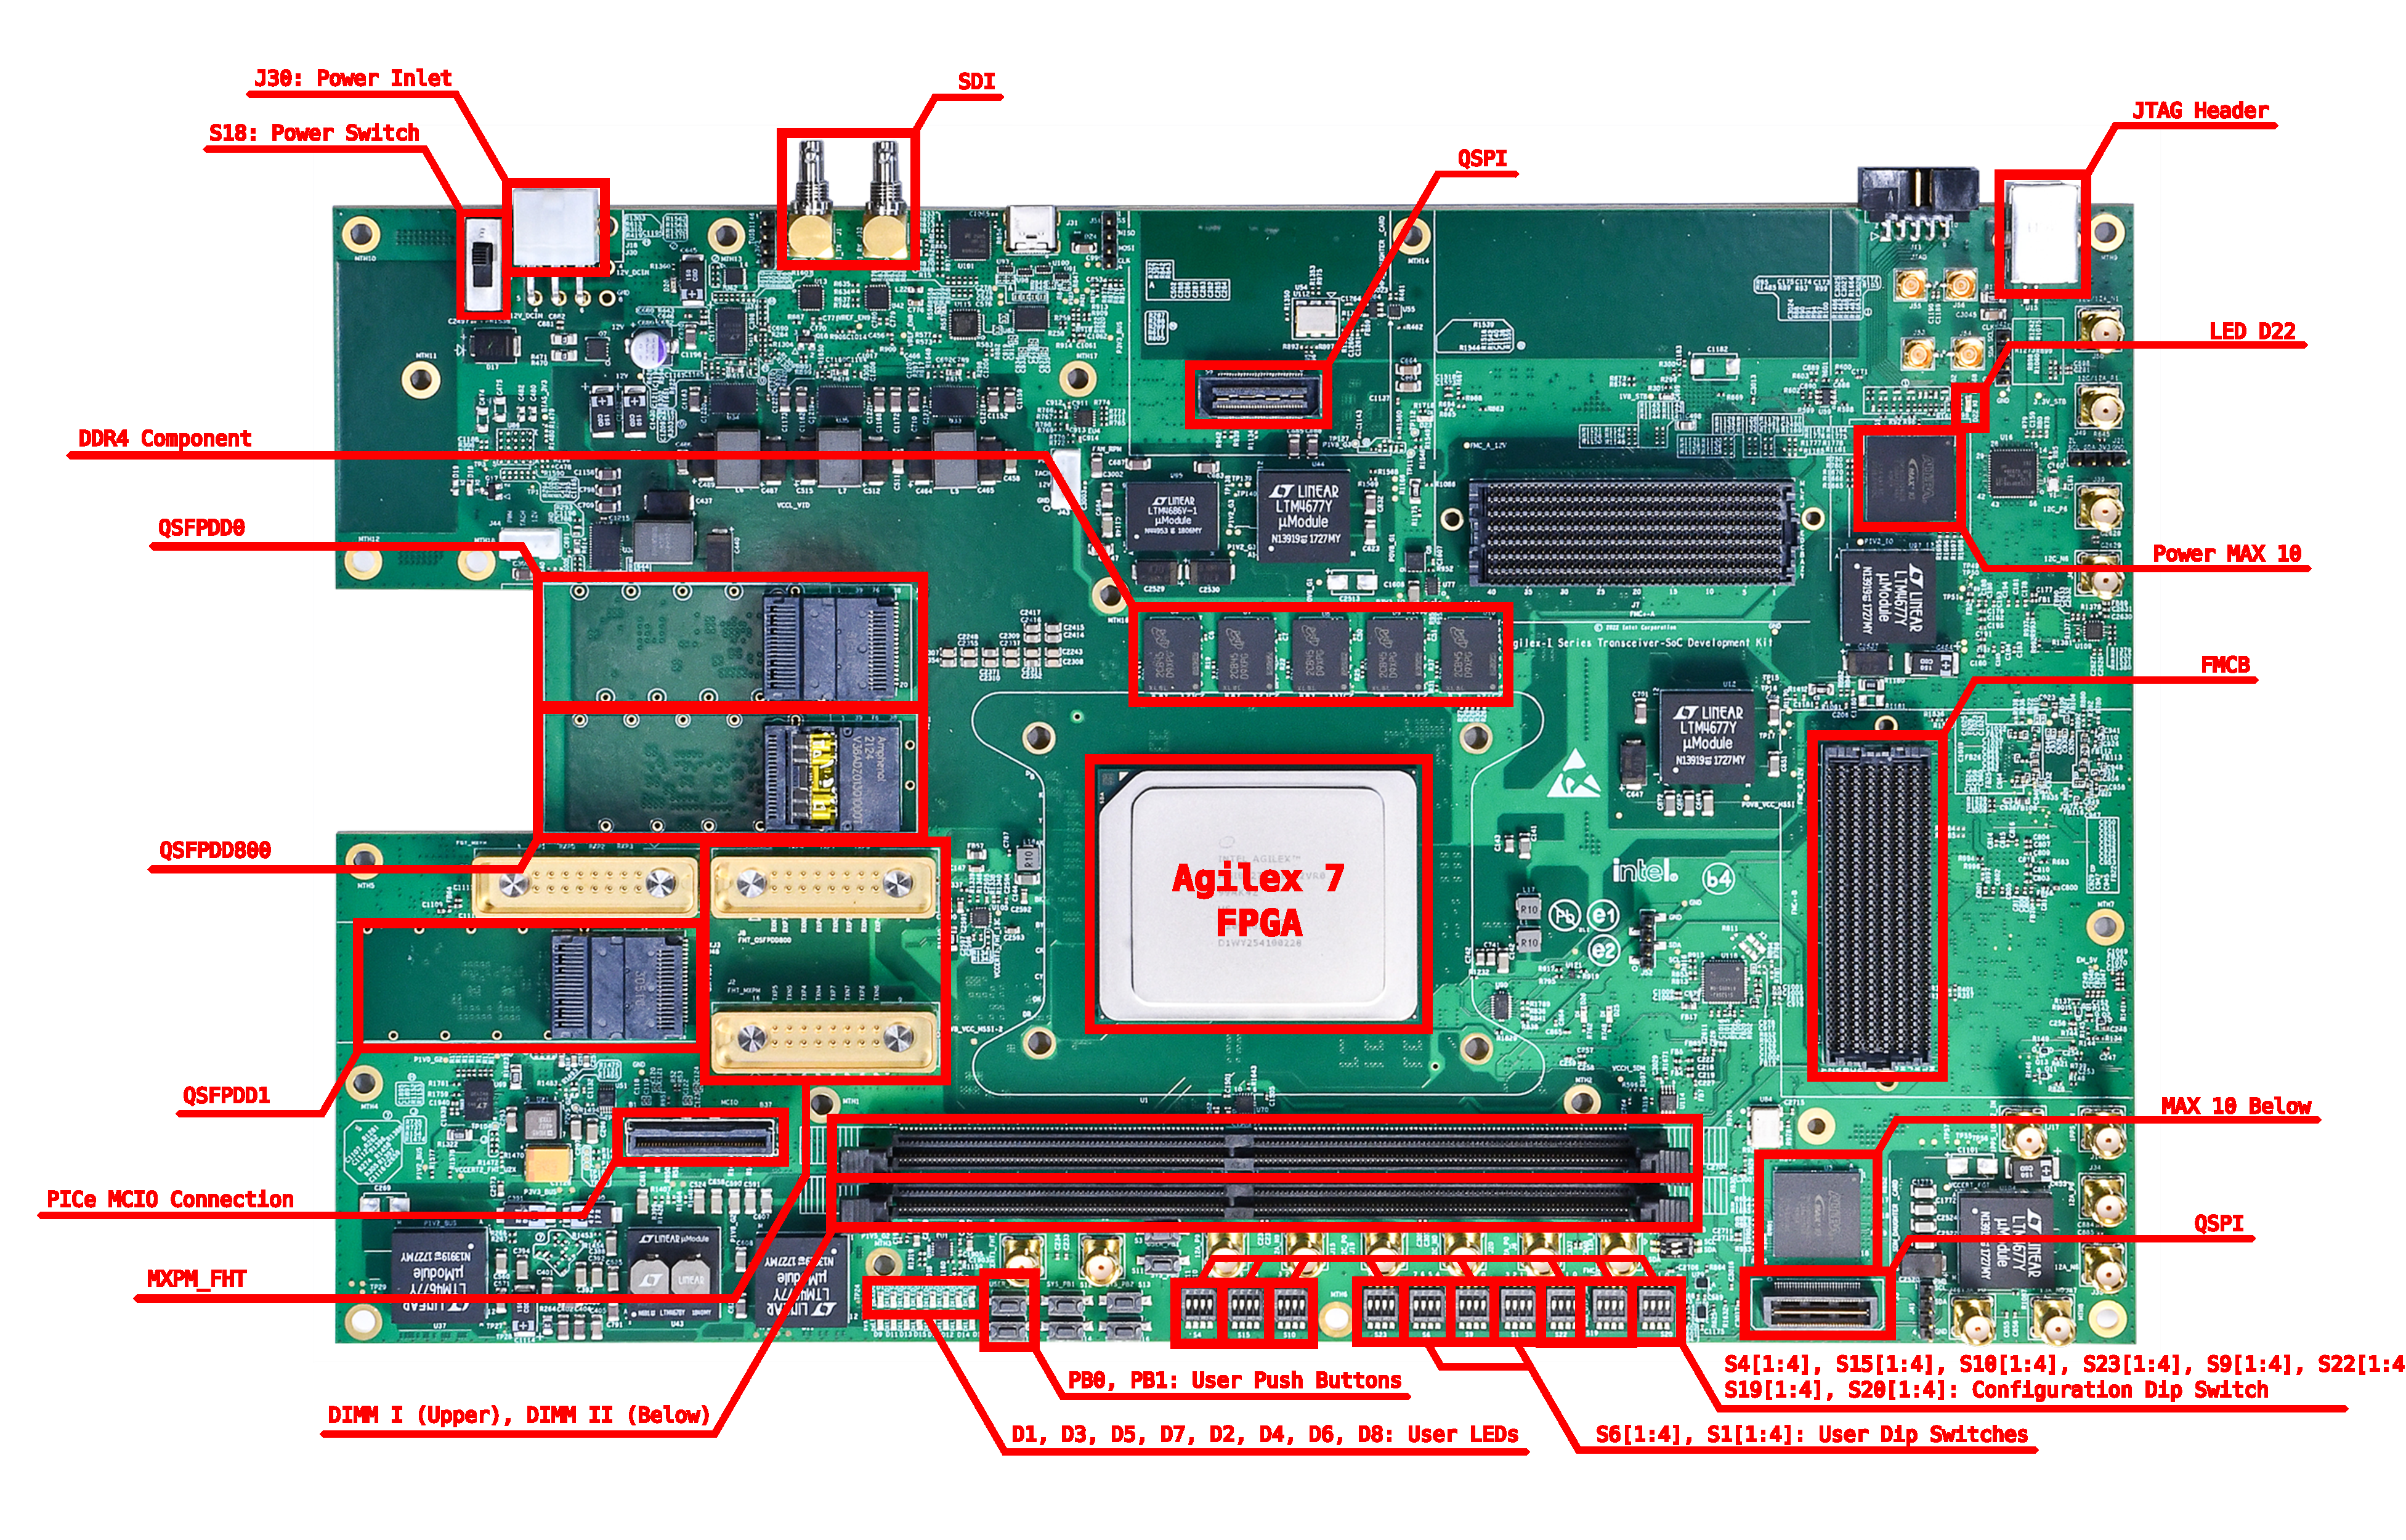
\includegraphics[width=\linewidth]{Images/Parte1/agilex7label.pdf}
        \caption{Elementos que integran a la tarjeta de desarrollo.}
        % \label{fig:enter-label}
    \end{figure}

\subsection{Resumen de caracter\'isticas}

\begin{itemize}
    \item Agilex 7 FPGA I-Series, 2.7M LE, 3184B package
    \begin{itemize}
        \item 2.7 millones de elementos l\'ogicos.
        \item Empaque tipo Ball Grid Array con 3184 bolas.
    \end{itemize}

    La tarjeta inlcuye m\'ultiples bancos de transceptores de alta velocidad (F-Tiles), dividididos en FHT y FGT.
    
    \item F-Tile 1 (13C)
    \begin{itemize}
        \item 4 canales transceptores FHT (F-Tile High-speed Transceiver) a QSFPDD800: transceptores para m\'odulos de fibra \'optica Quad Small Form-Factor Pluggable Double Density 800 (hasta 800 Gbps).
        \item 8 canales transceptores FGT (F-Tile General-purpose Transceiver) a QSFPDD: transceptores m\'as comunes, conectados a m\'odulos \'opticos QSFPDD.
        \item 2 canales transceptores FGT a HD-BNC: transmisi\'on de video (Serial Digital Interface).
        \item 4 transceptores FGT a DP2.0: Salida para DisplayPort 2.0.
        \item 1 transceptor FGT a USB3.2: Interfaz USB de alta velocidad.
    \end{itemize}
    \item F-Tile 2 (13A)
    \begin{itemize}
        \item 4 canales transceptores FHT (116G) a MXPM (Multi CoaX Press Mount): conectores de alta densidad para pruebas o backplanes.
        \item 8 canales transceptores FGT (56G) a MXPM.
        \item 8 canales transceptores FGT a QSFPDD.
        \item 4 canales transceptores FGT a MCIO (PCIe): interfaz PCI Express usando est\'andar Multi-Connector I/O.
    \end{itemize}
    \item F-Tile 3 (12C)
    \begin{itemize}
        \item 16 canales FGT a FMC+: permite conectar daughter cards por medio del est\'andar FPGA Mezzanine Card Plus para ampliar la funcionalidad.
    \end{itemize}
    \item F-Tile 4 (12A) 
    \begin{itemize}
        \item 16 canales FGT a FMC+.
    \end{itemize}
    \item SR DDR4 2666 (x72 w/ECC), 16 GB
    \begin{itemize}
        \item Memoria RAM DDR4 de 16 GB con Error Correcting Code y soporte para configuraciones de double rank (2DPC).
    \end{itemize}
    \item 8 GB SR DDR4-2666 (x72 w/ECC) dedicada al HPS.
    \item Interfaz IO48 para HPS Out of Box Experience (OOBE) daughter cards
    \begin{itemize}
        \item Intefaz de 48 pines para conectar tarjetas de desarrollo o pruebas r\'apidas del subsitema HPS.
    \end{itemize}
\textit{Nota: para m\'as informaci\'on sobre el HPS digirse a la secci\'on \hyperref[hpssec]{Hard Processor System (HPS)}}.
\end{itemize}

\subsection{Contenidos de la caja}

\begin{itemize}
    \item Agilex 7 FPGA I-Series Transceiver-SoC Development Kit
\item Modulo de memoria DDR4 DIMM (Single-rank)
\item QSPI flash daughter card: tarjeta secundaria con memoria flash QSPI preprogramada con im\'agenes de f\'abrica para configurar la FPGA.
\item HPS IO48 OOBE daughter card: Tarjeta secundaria que incluye interfaces Ethernet, USB, UART y GPIO para facilitar la evaluaci\'on del HPS.
\item NAND daughter card: Tarjeta secundaria con memoria NAND flash utilizada para almacenamiento adicional o configuraci\'on alternativa.
\item Cable USB 2.0 tipo B 
\item Cable Ethernet 
\item Fuente de alimentaci\'on de 240W y cables NA/EU/JP/UK 
\item Adaptador para fuente de poder ATX - 24 pines a 6 pines
\end{itemize}

    \begin{figure}[H]
        \centering
        \begin{subfigure}[b]{0.4\linewidth}
            \centering
            \includegraphics[width=\linewidth]{Images/Parte1/qspiflash.png}
            \caption{QSPI Flash Card.}
            % \label{sourcefpga}
        \end{subfigure} \hspace{1cm}
        \begin{subfigure}[b]{0.4\linewidth}
            \centering
            \includegraphics[width=\linewidth]{Images/Parte1/nandcard.png}
            \caption{NAND daughter card.}
            % \label{sourcefpga}
        \end{subfigure}
        \caption{Tarjetas hijas externas.}
        % \label{fig:enter-label}
    \end{figure}

\subsection{Condiciones de operaci\'on recomendadas}

\begin{table}[H]
    \centering
    \begin{tabularx}{\linewidth}{l|X}
        \toprule 
        \multicolumn{1}{c}{\textbf{Condición de operación}} & \multicolumn{1}{c}{\textbf{Rango de valores}} \\
        \toprule
        Rango de operación para temperatura ambiente & $0\degree$C a $30\degree$C \\ 
        \midrule
        Carga de corriente ICC & 195 A \\
        \midrule
        Porcentaje de carga transitorio ICC & 200 $A/\mu$s \\ 
        \midrule
        FPGA Máxima potencia soportada por disipador/ventilador activo & 160 $W$\footnotemark \\ 
        \bottomrule
    \end{tabularx}
    \caption{Condiciones de operación recomendadas.}
    \label{tab:my_label}
\end{table}
\footnotetext{160 $W$ para el núcleo y 60 $W$ para el transceptor FGT.}



   \section{Encendido de la tarjeta de desarrollo}

   Cuando se est\'a sosteniendo la tarjeta de desarrollo es muy importante tomar las precauciones adecuadas para no dañarla, ya que es susceptible a las descargas electroest\'aticas. 

   \begin{description}
       \item[\textbf{\textit{\textcolor{red}{Precauci\'on:}}}] La tarjeta puede ser dañada sin el manejo anti-descargas adecuado. Además, se deben usar precauciones anti-est\'atica cuando se toca la tarjeta.
       \item[\textbf{\textit{\textcolor{red}{Precauci\'on:}}}] Esta tarjeta de desarrollo no debe ser operada en un ambiente vibratorio.
   \end{description}

\subsection{Configuraci\'on de la tarjeta de desarrollo}

    Las instrucciones de esta secci\'on explican c\'omo configurar la tarjeta de desarrollo para el uso en casos espec\'ificos.

\subsection{Configuraci\'on predeterminada}

    La tarjeta de desarrollo Agilex 7 FPGA I-Series trae incluidos switches preconfigurados para soportar los ejemplos de diseño en el kit. Si se sospecha que la tarjeta de desarrollo no está configurada correctamente, sigue las instrucciones de la \ctref{tablasw} para regresar a la configuraci\'on predeterminada antes de avanzar.

    \begin{description}
        \item[\textit{Nota:}] ``X'' significa No Importa en la \ctref{tablasw}. 
        \item[\textit{Nota:}] No se deben de cambiar los switches de configuraci\'on cuando la tarjeta est\'a encendida, solamente cuando est\'a apagada.
    \end{description}

  \begin{longtable}{p{0.15\linewidth}|p{0.25\linewidth}|p{0.5\linewidth}} 
% \caption{Configuraci\'on por defecto de los switches de configuraci\'on.}
%   \label{tablasw}\\
            \toprule
             \multicolumn{1}{c}{\textbf{Switch}}&\multicolumn{1}{c}{\textbf{Posici\'on predeterminada}}&\multicolumn{1}{c}{\textbf{Funci\'on predeterminada}}\\ 
             \toprule
             \endfirsthead

            \toprule
             \multicolumn{1}{c}{\textbf{Switch}}&\multicolumn{1}{c}{\textbf{Posici\'on predeterminada}}&\multicolumn{1}{c}{\textbf{Funci\'on predeterminada}}\\ 
             \toprule
             \endhead
             
             S19[1:4]&OFF/OFF/ON/ON& Sistema Max 10 y FPGA seleccionada en la cadena JTAG. \\\midrule
             S20[1:4]&ON/ON/ON/ON& Modo 1: El circuito de descarga integrado de Intel actua como el \'unico JTAG maestro. HPS encadenado con nodos SDM internamente.\\\midrule
             S9[1:4]&ON/OFF/OFF/X&\parbox[t]{\linewidth}{Configuraci\'on de modo de carga de bits: AS - modo r\'apido.}\\\midrule
             S10[1:4]&ON/ON/ON/ON&
             \parbox[t]{\linewidth}{SYS\_SW[0:3]
             \begin{itemize}
                 \item SYS\_SW[0]-Factory Loadn
\item '0'-Load image from Page 0 of the
QSPI
\item SYS\_SW[1]-MUX\_SEL1
\item SYS\_SW[2]-MUX\_SEL7
\item SYS\_SW[3]-MUX\_SEL9\end{itemize}}\\\midrule
             S15[1:4]&ON/ON/ON/OFF&\parbox[t]{\linewidth}{SYS\_SW[4:7]
             \begin{itemize}
                 \item SYS\_SW[4]-MUX\_SEL\_ZL
\item SYS\_SW[5]-FMC-A PCIe RP/EP
Select
\begin{itemize}
    \item '0': RP (Default)
\item '1': EP
\end{itemize}
\item SYS\_SW[6]-FMC-B PCIe RP/EP
Select
\begin{itemize}
    \item '0': RP (Default)
\item '1': EP
\end{itemize}
\item SYS\_SW[7]-MCIO PCIe RP/EP
Select
\begin{itemize}
    \item '0': RP
\item '1': EP (Default)
\end{itemize}
\end{itemize}}\\\midrule

             S1[1:4]&OFF/OFF/OFF/OFF&Switch de usuario [0:3]\\\midrule
             S6[1:4]&OFF/OFF/OFF/OFF&\parbox[t]{\linewidth}{Switch de usuario [4:7]}\\\midrule
             
             S22[1:4]&ON/ON/ON/ON&\parbox[t]{\linewidth}{MUX\_DIP\_SW[0:3]
             \begin{itemize}
             \item MUX\_DIP\_SW0-MUX\_SEL2
\item MUX\_DIP\_SW1-MUX\_SEL3
\item MUX\_DIP\_SW2-MUX\_SEL4
\item MUX\_DIP\_SW3-MUX\_SEL5
             \end{itemize}}
             Puesto en ``ON'' por defecto para seleccionar el reloj integrado como entrada.
             \\\midrule
             
             S23[1:4]&ON/ON/ON/ON&
             \parbox[t]{\linewidth}{MUX\_DIP\_SW[4:7]
             \begin{itemize}
             \item MUX\_DIP\_SW4-MUX\_SEL10
\item MUX\_DIP\_SW5-MUX\_SEL11
\item MUX\_DIP\_SW6-MUX\_SEL12
\item MUX\_DIP\_SW7-MUX\_SEL14
             \end{itemize}}
             Puesto en ``0''/cerrado por defecto para el reloj integrado como entrada.
             \\\midrule
             S4[1:4]&ON/ON/ON/ON&
             \parbox[t]{\linewidth}{MUX\_DIP\_SW[8:11]
             \begin{itemize}
             \item MUX\_DIP\_SW8-MUX\_SEL13
\item MUX\_DIP\_SW9-MUX\_SEL6
\item MUX\_DIP\_SW10-MUX\_SEL0
\item MUX\_DIP\_SW11-MUX\_SEL8
             \end{itemize}}
             Puesto en ``0''/cerrado por defecto para el reloj integrado como entrada.
             \\\bottomrule

             \caption{Configuraci\'on por defecto de los switches de configuraci\'on.}
        \label{tablasw}
        \end{longtable}
        

\subsection{Encendido}

        Para el correcto encendido de la tarjeta debemos realizar los siguientes pasos:
        \begin{enumerate}
            \item Usa el adaptador de alimentaci\'on de 240 $W$ para suministrar alimentaci\'on a trav\'es de \texttt{\textcolor{red}{J30}}.
            \item Despu\'es de que el adaptador de alimentaci\'on est\'a conectado en \texttt{\textcolor{red}{J30}} y el switch \texttt{\textcolor{red}{S18}} est\'a en la posici\'on de ON el LED \texttt{\textcolor{red}{D22}} se enciende, indicando que la tarjeta se encendio correctamente. Si el LED \texttt{\textcolor{red}{D22}} no se enciende, significa que una o m\'as fuentes de alimentaci\'on son incorrectas.
        \end{enumerate}
        \textit{Nota: Al encender la tarjeta los ventiladores generan bastante ruido, sin embargo esto es normal y no debe generar preocupaci\'on}.
    
        \begin{figure}[H]
            \centering
            \begin{subfigure}[b]{0.4\linewidth}
                \centering
                \includegraphics[width=\linewidth, clip, trim=7cm 6cm 7cm 4cm ]{sourcefpga.png}
                \caption{Entrada de alimentaci\'on a el FPGA.}
                \label{sourcefpga}
            \end{subfigure}
            \hspace{.5cm}
            \begin{subfigure}[b]{0.4\linewidth}
                \centering
                \includegraphics[width=\linewidth, clip, trim=9cm 7cm 7cm 4.5cm ]{jtagfpga.png}
                \caption{Conexi\'on USB JTAG para el programador.}
                \label{jtagfpga}
            \end{subfigure} 

            
            \begin{subfigure}[b]{0.4\linewidth}
                \centering
            \includegraphics[width=\linewidth, clip, trim=13cm 8cm 7cm 6cm]{switch.png}
            \caption{Posici\'on de apagado para el switch de encendido.}
            \label{fig:switch}
            \end{subfigure}
            
            \caption{Conexi\'on de alimentaci\'on y USB JTAG a la tarjeta y encendido de la tarjeta.}
            \label{fig:conexion}
        \end{figure}

\section{Reinicio de la tarjeta de desarrollo}

    Esta tarjeta de desarrollo inicia con los diseños de ejemplo \curl{bts_config} almacenadas en el dispositivo de memoria flash QSPI. El proceso de reinciar la tarjeta a su configuraci\'on de f\'abrica consiste en grabar el contenido original en el MAX 10, que supervisa el sistema, y la memoria flash QSPI, donde se guarda la configuraci\'on de arranque del FPGA.\\ 
    
    Se puede realizar el reinicio de la tarjeta siguiendo las siguientes instrucciones a trav\'es de la interfaz Quartus Prime Programmer GUI.

\subsection{Reiniciar el MAX 10 con la im\'agen de f\'abrica}

El MAX 10 es un FPGA que controla el encendido del sistema, JTAG, monitoreo de voltajes, entre otras funciones. Para grabar los contenidos originales hay que seguir los siguientes pasos.

\begin{enumerate}
    \item Abrir Quartus Prime Programmer GUI y detectar la cadena JTAG despu\'es de que System MAX 10 es almacenado.
    \item Adjunta la imagen de System MAX 10 en la parte System MAX 10.
    \item Seleccionar opciones de programaci\'on y dar click en el bot\'on de programar.
\end{enumerate}

\textit{Nota: Una vez que se conecta el cable de descarga FPGA entre} \texttt{\textcolor{red}{J11}} \textit{y la estaci\'on de trabajo, se desactiva autom\'aticamente el circuito de descarga integrado en la placa.}

\subsection{Reinicio de la memoria flash QSPI con la imagen de f\'abrica}

    La memoria flash QSPI est\'a pre-programada con 4 paquetes de im\'agenes. Los pasos siguientes indican como sobreescribir la imagen de modo de configuraci\'on de la interfaz de transmisi\'on Avalon x8.

    \begin{enumerate}
        \item Asegurarse que MSEL[2:0] est\'a apagado (modo JTAG) antes de encender la tarjeta.
        \item Abrir Quartus Prime Programmer GUI y detectar la cadena JTAG.
        \item Cambiar el dispositivo VTAP10 a 10M50DAF256, adjuntar el dispositivo flash de QSPI\_2Gb.
        \item Adjuntar el archivo de configuraci\'on para el modo Avalon Streaming interface x8 a QSPI\_2Gb.
        \item Seleccionar las opciones Programar/Configurar y dar click en el bot\'on \texttt{\textcolor{DarkOrchid1}{Start}}.
        \item Despu\'es de programar la memoria flash apagar la tarjeta y cambiar MSEL[2:0] OFF OFF ON (modo de configuraci\'on por Avalon Streaming interface x8).
    \end{enumerate}